\section{ОСОБЕННОСТИ РЕАЛИЗАЦИИ}
\addcontentsline{toc}{section}{Особенности  реализации}

В данном разделе описаны детали реализации приложения, а также приведены результаты его тестирования.
В ходе работы над проектом необходимо было реализовать модульные компоненты, которые позволили
бы в дальнейшем минимизировать трудозатраты на доработки и расширение системы.

\subsection{Обоснование выбора средств и методов разработки}

Использование современных технологий при разработке платформы должно позволять
с минимальными затратами расширять данную систему под нужды конкретного университета.
При разработке программного обеспечения для серверной части был выбран
язык программирования Python совместно с Django.
Django - это свободный фреймворк для веб-приложений, использующий шаблон проектирования MVC.
Данный фреймворк является не только быстрым решением в веб разработке,
включающим все необходимое для качественного кода и прозрачного написания,
но также и отличной платформой для работы с клиентурой того или иного бизнеса,
а также разработчиков. С помощью Django можно гибко настроить панель управления контентом
(админку сайта) под любой конкретный проект - управление видеоматериалами,
комментариями и пользовательскими данными в данном случае.

Обработка видео является трудоемкой задачей, для которой требуется большое количество временных
и вычислительных ресурсов. Такого рода манипуляции не требуют участия конечного пользователя
вашего проекта, то есть их можно выполнять в фоновом режиме. При этом важно,
чтобы весь процесс оставался управляемым.

\begin{figure}
  \centering
  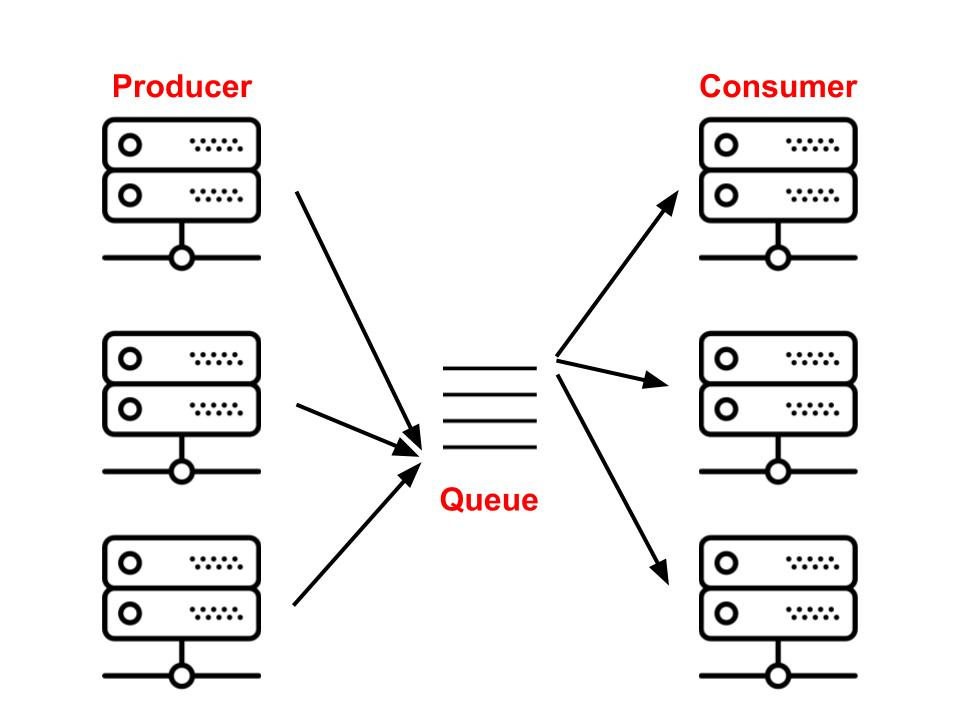
\includegraphics[width=0.8\textwidth]{images/producer-consumer.jpg}
  \caption{Очередь обработки видеофайлов\label{producer-consumer}}
\end{figure}

На рисунке \ref{producer-consumer} представлена общая схема очереди обработки видеофайлов.
Файлы, загруженные пользователями (“Producer” на схеме) из разных мест,
поступают в единую очередь “Queue”. Далее они обрабатываются обработчиками (“Сonsumer” на схеме)
в порядке поступления в очередь. Обработчик очереди может быть и один.
Для нашего приложения важно, чтобы очередь поддерживала следующий функционал:
\begin{itemize}
  \item выполнение заданий асинхронно или синхронно;
  \item выполнение периодических заданий;
  \item выполнение задание повторно, если произошла ошибка;
  \item мониторинг выполнения заданий;
  \item проверка выполнения задания (уведомить пользователя о том, что видео прошло обработку).
\end{itemize}

В разработанном приложении было решено использовать распределенную очередь Celery,
которая является одним из самых популярных проектов для решения подобных задач в мире
python и Django. Это распределенная асинхронная очередь заданий, которая обладает
перечисленным выше функционалом, легко интегрируема и удобна в использовании.

Скорость загрузки любого сайта достаточно важный и существенный параметр, который определяет
качество и надежность ресурса. Для образовательной платформы это вдвойне важно. При просмотре
видео не должны возникать существенные задержки в загрузке контента, иначе это негативно
скажется на общем впечатлении пользователей. Оптимизировать сайт можно многими способами,
и если каждый из них уже себя исчерпал, нужно подключать сторонние сервисы в помощь, например,
сервис CDN. Данная аббревиатура расшифровывается как Content Delivery Network – сеть доставки
контента. Чаще всего это множество серверов со специализированным ПО, которые ускоряют доставку
(“отдачу”) контента конечному пользователю. Сервера расположены по всему миру таким образом,
чтобы время ответа посетителям сайта было минимальным. Под “контентом” чаще всего
подразумевают видео и статические элементы веб-сайтов (не требующие выполнения кода на сервере
или запросов в базу данных, такие как css/js).

\begin{figure}
  \centering
  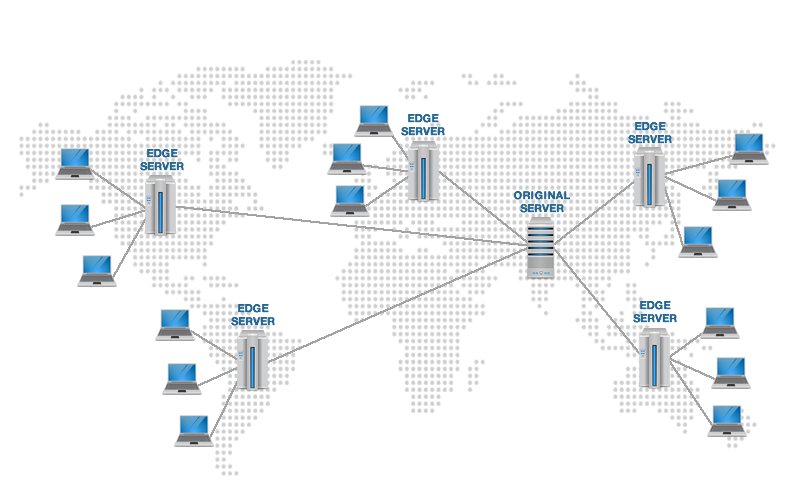
\includegraphics[width=0.9\textwidth]{images/how-cdn-works.png}
  \caption{Content Delivery Network\label{how-cdn-works}}
\end{figure}

На рисунке \ref{how-cdn-works} представлена одна из возможных схем распределения серверов CDN по миру.
Все современные CDN размещают копии контента на разных серверах по всему миру и направляют
клиента на ближайший (к клиенту) сервер. Результат — сокращение “latency”, то есть задержки
между запросом и ответом. Если на странице много изображений (пусть даже мелких картинок),
то чем быстрее они окажутся у клиента, тем быстрее клиент увидит страницу.

В разработанном приложении в качестве CDN было решено использовать Amazon CloudFront.
Это это удобный для разработчиков сервис глобальной сети доставки контента, обеспечивающий
быструю и безопасную передачу данных, видео, приложений и API клиентам по всему миру
с низкими задержками и высокой скоростью.